\chapter{Abordagem Proposta}
\label{cap:abordagem_proposta}

Para o desenvolvimento deste trabalho, propõe-se quatro etapas principais que seguem a estrutura padrão adotada pelos trabalhos analisados, conforme ilustrado na Figura \ref{fig:abordagemPadrao}. Inicialmente, é realizada a construção do conjunto de dados, cujos processos são descritos em detalhes na Seção \ref{sec:base_dados}. Em seguida, ocorre a seleção de variáveis relevantes, abordada na Seção \ref{sec:selecao_variaveis}. Com as variáveis selecionadas, inicia-se o processo de previsão, que é detalhado na Seção \ref{sec:previsao}. Por fim, é realizada a recomendação de investimento com base nos valores previstos, conforme descrito na Seção \ref{sec:estrategia}. 

\section{Construção dos Conjuntos de Dados}
\label{sec:base_dados}
O processo de construção do conjunto de dados é dividido em duas etapas distintas. Primeiramente, ocorre a extração dos dados, conforme detalhado na Seção \ref{subsec:extracao}. Em seguida, é realizada a geração de novas variáveis a partir dos dados extraídos, como explicado na Seção \ref{subsec:feature_generate}. Nessa fase, são criadas variáveis adicionais que fornecem informações relevantes para o processo de previsão e análise. A Figura \ref{fig:base_dados} apresenta uma visão geral do processo de construção do conjunto de dados, ilustrando de forma visual as etapas mencionadas. Esse processo garante a disponibilidade dos dados necessários e a preparação adequada das variáveis para as etapas subsequentes do trabalho.

\begin{figure}[htbp]
    \caption{Visão macro do processo de construção do conjunto de dados.}
      \centering
    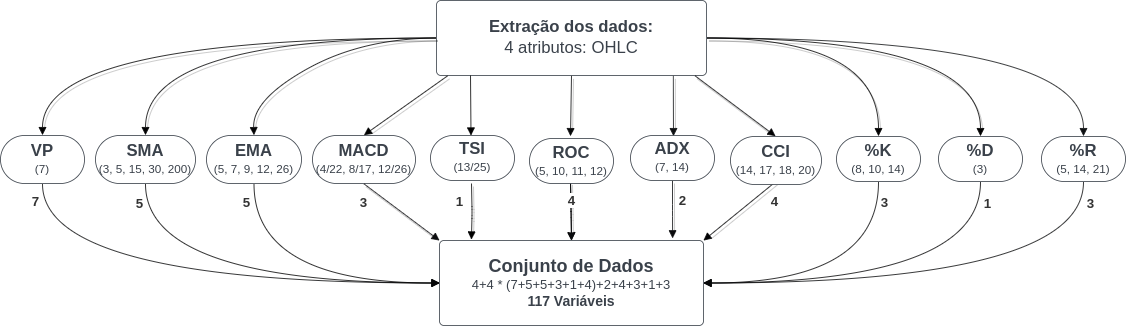
\includegraphics[width=.99\linewidth]{base_dados.png} 
    \label{fig:base_dados}
\end{figure}


\subsection{Extração de Atributos}
\label{subsec:extracao}
O mercado de ações do Brasil possui um horário de funcionamento de segunda a sexta-feira, das 10:00 às 17:00 \cite{B3H:2023}. Durante esse período, são geradas informações em diferentes granularidades, permitindo acompanhar a evolução dos preços e volumes de negociação ao longo do tempo. Uma plataforma amplamente utilizada para acessar essas informações é o \textit{Investing}\footnote{https://www.investing.com}, que disponibiliza dados históricos e em tempo real em diferentes intervalos, como diário, semanal e mensal. Essa plataforma abrange diversos mercados e modalidades de investimento em vários países, fornecendo informações relevantes, como os preços de abertura, máxima, mínima, fechamento (OHLC), volume negociado e percentual de mudança. É importante mencionar que existem outras fontes disponíveis para a coleta de dados, como a plataforma \textit{Profit}\footnote{https://www.nelogica.com.br/produtos/profit-ultra}, a B3\footnote{https://www.b3.com.br/pt\_br/market-data-e-indices/servicos-de-dados/market-data/historico/}, entre outras. No contexto deste trabalho, os dados históricos \ac{OHLC} foram extraídos da plataforma \textit{Profit} para análise e estudo.

\subsection{Geração de Variáveis}
\label{subsec:feature_generate}
Após a extração dos dados, são aplicadas diversas técnicas para gerar variáveis relevantes na tarefa de previsão. Para esse propósito, são calculadas novas variáveis a partir de cada valor de \ac{OHLC}, utilizando diferentes fórmulas econômicas ajustadas a parâmetros específicos abordados na literatura. Essas técnicas visam extrair informações adicionais dos dados e incluem:
\begin{itemize}
    \item \ac{VP} - é obtido por meio do deslocamento de 7 valores passados \cite{Vinícius_Sistemas};

    \item \ac{SMA} - calculada a partir da Equação (\ref{eq:SMA}) empregada aos intervalos de 3 \cite{chantarakasemchit2020forex}, 5, 15, 30 \cite{handayani2019longer} e 200 \cite{ELLIS2005399};
    
    \item \ac{EMA} - tem seu calculo baseado na Equação (\ref{eq:EMA}), sendo aplicada aos períodos amostrais de 5, 7, 9 \cite{ANBALAGAN2015214}, 12 \cite{Charlene} e 26 \cite{ananthi2021retracted};
    
    \item \ac{MACD} - derivado da Equação (\ref{eq:MACD}) aplicada aos valores de janela móvel curta e janela móvel longa como 12/26 \cite{ANBALAGAN2015214, handayani2019longer}, 8/17 e 4/22 \cite{kang2021improving}, respectivamente;
    
    \item \ac{CCI} - calculado a partir da Equação (\ref{eq:CCI}), considerando os períodos de amostragem de 14 \cite{halil2019predicting}, 17, 18 \cite{karasu2022crude} e 20 \cite{kelotra2020stock} para a janela de análise;
    
    \item \ac{ADX} - obtido através da Equação (\ref{eq:ADX}) aplicada aos períodos de 7 \cite{kelotra2020stock} e 14 \cite{shamseddin2022mapping} espaços amostrais;
    
    \item \ac{ROC} - determinado a partir da Equação (\ref{eq:ROC}) empregada aos intervalos de 5, 10, 11 e 12 \cite{karasu2022crude};
    
    \item \ac{TSI} - computado a partir da Equação (\ref{eq:TSI}) com base  nos intervalos de 13 para a janela móvel curta e 25 para a janela móvel longa \cite{nayak2015naive, anwar2019forecasting};
    
    \item \ac{K} - calculado com base na Equação (\ref{eq:K}) utilizando os intervalos de tempo de 8 \cite{ni2022does}, 10 \cite{ijegwa2014predictive} e 14 amostras \cite{C_Veeramani_Exploration};
    
    \item \ac{D} - derivado da Equação (\ref{eq:D}) aplicada a janela de tempo de 3 amostras \cite{ijegwa2014predictive, vaidya2018stochastic};
    
    \item \ac{R} - tem seu calculo baseado na Equação (\ref{eq:R}), considerando as janelas de tempo de 5, 14 e 21 espaços amostrais \cite{de2016multi}.
\end{itemize}

Como resultado desse processo, são geradas um total de 117 variáveis, o que proporciona uma variedade de padrões de entrada para os modelos de previsão.



\section{Seleção de Variáveis}
\label{sec:selecao_variaveis}
Com a base de dados gerada, é importante ressaltar que nem todas as variáveis possuem a mesma relevância para o processo de previsão, pois essa relevância pode depender tanto do objetivo do processo de previsão quanto dos modelos utilizados. Portanto, é necessário realizar a seleção de variáveis, a qual foi dividida em duas etapas neste estudo. Primeiramente, são empregados alguns métodos de seleção de variáveis descritos na Seção \ref{subsec:selecao_variaveis}. Em seguida, as variáveis selecionadas são agrupadas e classificadas em dois conjuntos de dados distintos, denominados \textit{Dataset-1} e \textit{Dataset-2}. Uma representação geral desse processo pode ser observada na Figura \ref{fig:feature_selection}.

\begin{figure}[htbp]
    \caption{Visão macro do processo de seleção de variáveis.}
      \centering
    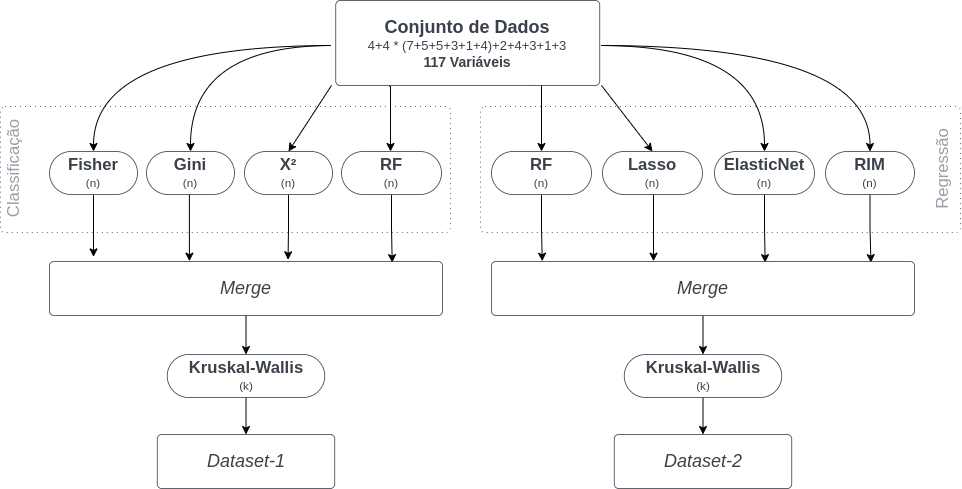
\includegraphics[width=.99\linewidth]{feature_selection.png} 
    \label{fig:feature_selection}
\end{figure}

Na primeira etapa do processo de seleção de variáveis, são aplicados dois grupos de algoritmos. O primeiro grupo é direcionado para modelos de classificação e inclui os métodos de Fisher, Gini, \ac{R2} e \ac{RF}. Enquanto o segundo grupo é direcionado para modelos de regressão e inclui os métodos de \ac{RF}, Lasso, ElasticNet e \ac{RIM}. Cada um desses métodos, pertencentes aos dois grupos, seleciona $n$ variáveis relevantes para a classificação ou regressão, respectivamente. 

Por fim, na segunda etapa do processo de seleção de variáveis, é realizado um \textit{merge} em cada grupo, unificando as variáveis selecionadas por cada método de seleção, sem que haja repetição. Em seguida, é aplicado o teste de \textit{Kruskal-Wallis} em cada grupo para ranquear as variáveis mais relevantes provenientes do \textit{merge}. Isso resulta em dois conjuntos de dados com $k$ variáveis cada: o \textit{Dataset-1}, referente ao grupo de classificação, e o \textit{Dataset-2}, referente ao grupo de regressão. O uso do modelo de \textit{Kruskal-Wallis} permite ordenar as variáveis de acordo com sua relevância, considerando as características específicas de cada grupo. Essa etapa visa consolidar os conjuntos de dados finais, contendo as variáveis mais importantes para cada tipo de tarefa, otimizando assim o processo de previsão.




\section{Máquina de Previsão}
\label{sec:previsao}
Para a construção da máquina de previsão proposta, foram empregadas duas técnicas de \textit{ensemble}: o \textit{Soft Voting} e o \textit{Stacking}. A Figura \ref{fig:model_prediction} ilustra a forma como essas técnicas foram integradas.

O \textit{Soft Voting}, conforme descrito por \citeonline{wang2013soft}, realiza uma votação ponderada, expressando a saída em percentuais correspondentes a cada classe. Nessa abordagem, diversos modelos são treinados de forma independente e suas previsões são combinadas usando pesos. O resultado final é obtido por meio de uma média ponderada das previsões de cada modelo, refletindo a confiança individual atribuída a cada classe.
Já o método conhecido como \textit{Stacking}, empregado por \citeonline{dietterich2002ensemble}, consiste na criação de camadas de modelos de predição interconectados. Nessa abordagem, os modelos de base são treinados coletivamente, e suas saídas são empregadas como entrada para um meta-modelo responsável pelo resultado final. O objetivo é combinar as previsões dos modelos de base de maneira a obter uma estimativa mais precisa e confiável.

\begin{figure}[htbp]
    \caption{Visão macro do processo de previsão.}
      \centering
    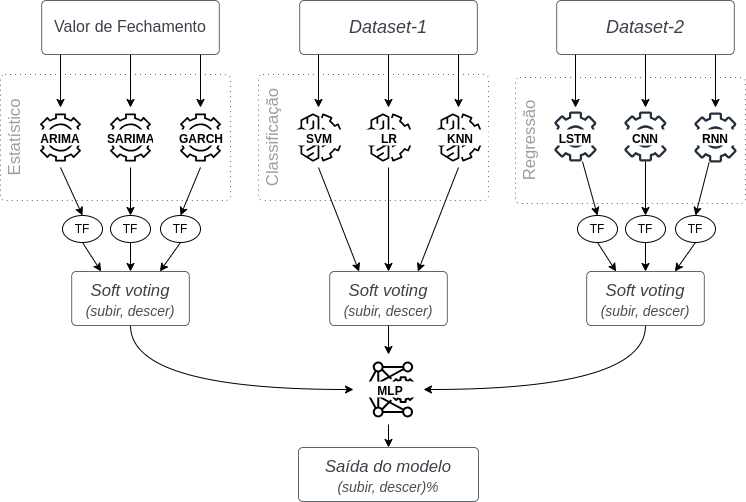
\includegraphics[width=.99\linewidth]{model_prediction.png} 
    \label{fig:model_prediction}
\end{figure}

Na abordagem proposta, são construídos três grupos de algoritmos distintos para a tarefa de previsão. O primeiro grupo consiste em modelos estatísticos, como por exemplo\ac{ARIMA}, \ac{SARIMA} e \ac{GARCH}, que utilizam apenas o valor de fechamento de cada amostra como entrada e possuem uma função de transformação na saída de cada modelo, conforme descrita na Tabela \ref{tab:RegraTransf}. O segundo grupo é composto por técnicas de \ac{IA} voltadas para classificação, como por exemplo \ac{SVM}, \ac{LR} e \ac{KNN}, que recebem como entrada o \textit{Dataset-1}, composto pelas variáveis relevantes selecionadas para tarefa de classificação. O terceiro grupo é formado por algoritmos de \ac{IA} voltados para regressão, como por exemplo \ac{LSTM}, \ac{RNN} e \ac{CNN}, que recebem como entrada o \textit{Dataset-2}, contendo as variáveis relevantes selecionadas para a tarefa de regressão e também possuem uma função de transformação na saída de cada modelo, de acordo com a Tabela \ref{tab:RegraTransf}. 

Em continuidade, as técnicas de \textit{Soft Voting} e \textit{Stacking} são aplicadas de forma sequencial. O \textit{Soft Voting} combina as previsões de cada grupo de modelos, considerando a contribuição de cada um deles. Isso resulta em dois valores, sendo o graus de pertinência das classes 'subir' e 'descer'. Por sua vez, o \textit{Stacking} utiliza um algoritmo de \ac{IA} para combinar as saídas do \textit{Soft Voting} de cada grupo, resultando em duas saídas referentes aos percentuais de correlação a cada classe. 
Por exemplo, considere três modelos de previsão pertencentes ao mesmo grupo, que prevêem as classes 1, 0 e 1, respectivamente. Utilizando um sistema de \textit{soft voting}, as classes preditas pelos modelos são ponderadas, resultando em aproximadamente 66,5\% de chance da próxima amostra pertencer à classe 1 e 33,5\% de chance de pertencer à classe 0. Esse processo é repetido para cada conjunto de algoritmo: Estatístico, Classificação e Regressão. Em seguida, outro modelo genérico de IA recebe os percentuais de pertencimento de cada classe provenientes de cada conjunto de algoritmos, resultando em 6 entradas. Com base nessas 6 entradas, o modelo utilizado retorna dois valores: o percentual de pertencimento à classe 0 e 1.

\section{Recomendação de Investimento}
\label{sec:estrategia}

Tendo em mãos o percentual de subida ou descida obtido pela máquina de previsão proposta, inicia-se o processo de recomendação de compra e venda, conforme ilustrado na Figura \ref{fig:strategy}, que objetiva reduzir operações de baixa confiabilidade e maximizar os retornos financeiros. A estratégia de recomendação é baseada nos resultados da máquina de previsão, visando identificar oportunidades de investimento com maior probabilidade de sucesso.

\begin{figure}[htbp]
    \caption{Visão macro do processo de recomendação de investimentos.}
      \centering
    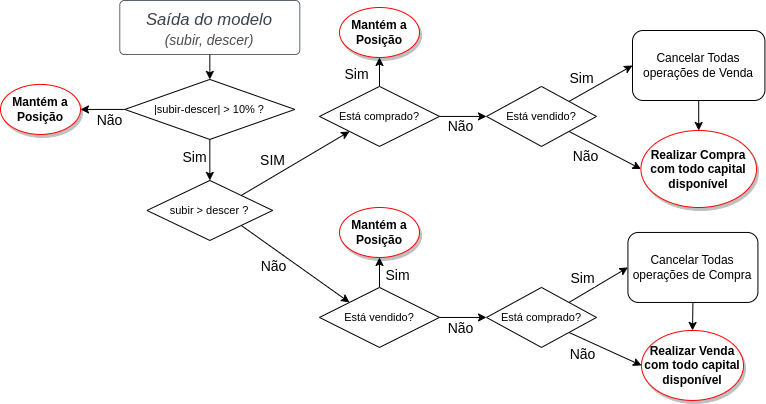
\includegraphics[width=.9\linewidth]{strategy.png} 
    \label{fig:strategy}
\end{figure}


A estratégia de recomendação inicia com um filtro para verificar se a diferença percentual entre as classes de subida e descida é relevante. Isso é feito calculando a diferença nos graus de pertencimento a cada classe. Se a diferença não for significativa, ou seja, menor que 10\%, a recomendação é não realizar nenhuma operação e manter a posição atual.
Caso a diferença seja significativa, é feita uma comparação entre os sinais de 'subir' e 'descer' para determinar qual classe apresenta um percentual de pertinência maior. Isso ajuda a identificar a direção mais provável do próximo valor.

Se o sinal de subida for considerado mais relevante, ou seja, a classe 'subir' tem um percentual de pertinência maior, a estratégia sugere que a probabilidade de o próximo valor ser maior do que o atual é alta. Nesse caso, é verificado se há recurso disponível na carteira de investimentos. Se houver recurso disponível, a recomendação é realizar a compra do ativo. Caso contrário, não é feita nenhuma ação.

Por outro lado, se o sinal de subida não for superior ao de descida, é mais provável que o próximo valor seja menor do que o atual. Nesse cenário, é verificado se há algum ativo já comprado. Se houver ativos comprados, a recomendação é vender todos eles, indicando uma posição defensiva para evitar perdas potenciais. Caso não haja ativos comprados, nenhuma ação é recomendada.